\documentclass[a4paper, 12pt]{article}

\usepackage{hyperref}
\usepackage[warn]{mathtext}
\usepackage[utf8]{inputenc}
\usepackage[T2A]{fontenc}
\usepackage[english,russian]{babel}
\usepackage{multirow}
\usepackage{amsmath,amsfonts,amssymb,amsthm,mathtools}
\usepackage{indentfirst}
\DeclareSymbolFont{T2Aletters}{T2A}{cmr}{m}{it}
\usepackage{ gensymb }
\mathtoolsset{showonlyrefs=true}
\usepackage{euscript}
\usepackage{mathrsfs}
\usepackage[left=2cm,right=2cm,top=2cm,bottom=2cm]{geometry}
\usepackage{graphicx}
\usepackage{wrapfig}
\usepackage[rgb]{xcolor}
\hypersetup{
colorlinks=true,
urlcolor=blue
}


\title{Лабораторная работа 1.3.3}
\author{Гисич Арсений Б03-109}
\date{2022}

\begin{document}

	\begin{center}
		{\large МОСКОВСКИЙ ФИЗИКО-ТЕХНИЧЕСКИЙ ИНСТИТУТ (НАЦИОНАЛЬНЫЙ ИССЛЕДОВАТЕЛЬСКИЙ УНИВЕРСИТЕТ)}
	\end{center}
	\vspace{5 cm}
	{\Large
		\begin{center}
			{\bf Лабораторная работа 2.3.1}\\[0.2 cm]
			Получение и измерение вакуума
		\end{center}
	}
	\vspace{4 cm}
	\begin{flushright}
		{\Large Выполнил: \\
			\vspace{0.2 cm}
			Гисич Арсений \\
			\vspace{0.2 cm}
			Б03-109 \\}
	\end{flushright}
	\vspace{9 cm}
	\begin{center}
		Долгопрудный\\[0.1 cm]
		2022
	\end{center}
\thispagestyle{empty}

\section{Аннотация}

\par Цель работы: 1) измерение объемов форвакуумной и высоковакуумной частей установки; 2) определение скорости откачки системы в стационарном режиме, а также по ухудшению и улучшению вакуума.

\section{Теоретические сведения}

В физике вакуумом называют состояние газа, при котором характерная длина свободного пробега молекул в газе $\lambda$ сравнима по порядку
величины с характерным линейным размером сосуда $d$, в котором газ
находится. Для воздуха при нормальных условиях $\lambda \sim 10^{-5}~см$, откуда
видно, что воздух в жилых помещениях не находится в состоянии вакуума, но, например, внутри пористых материалов, таких как древесина, уже
может находиться.

В технике вакуумом называют состояние газа при котором его
давление меньше атмосферного ($P < P_{атм}$). Различают следующие типы
вакуума: \textit{низкий}, когда средняя длина свободного пробега молекул газа
значительно меньше характерного линейного размера рассматриваемого
объёма, т.е. $\lambda < d$; \textit{средний}, когда $\lambda \sim d$; \textit{высокий} (или глубокий), когда
$\lambda \gg d$ (рис. \ref{ris1}). Иногда выделяют ещё \textit{сверхвысокий} вакуум, при котором
не происходит заметного изменения свойств поверхности, первоначально
свободной от адсорбированного газа, за время, существенное
для проведения эксперимента. Газ в состоянии высокого вакуума называется \textit{ультраразреженным}.

\begin{figure}[h!]
	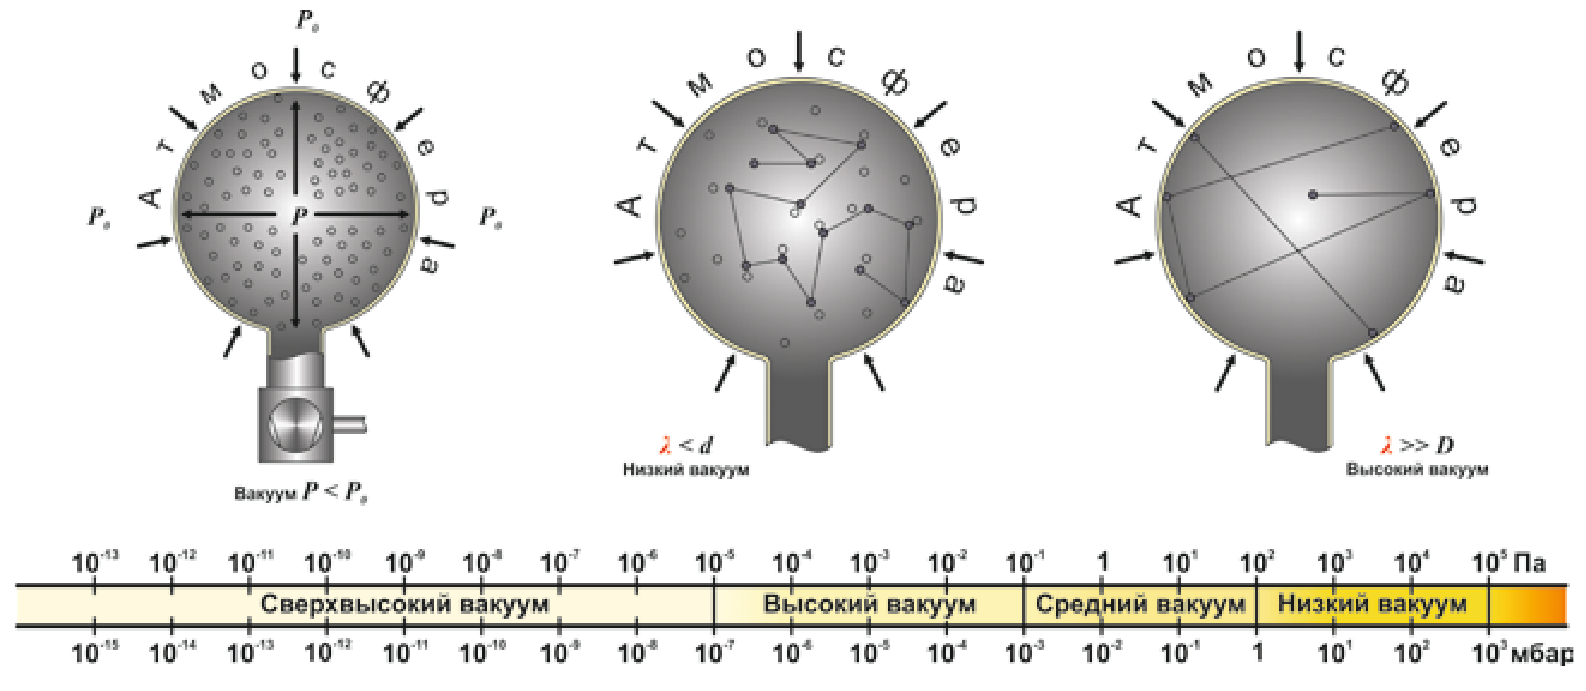
\includegraphics[width = \textwidth]{1.png}
\caption{Понятие о вкаууме}
\label{ris1}
\end{figure}

\subsection{Некоторые понятия для работы с вакуумной техникой}

Основы процесса откачки и связанные с ним понятия рассмотрим на примере простейшей вакуумной системы (рис. \ref{ris2}).

\begin{figure}[h!]
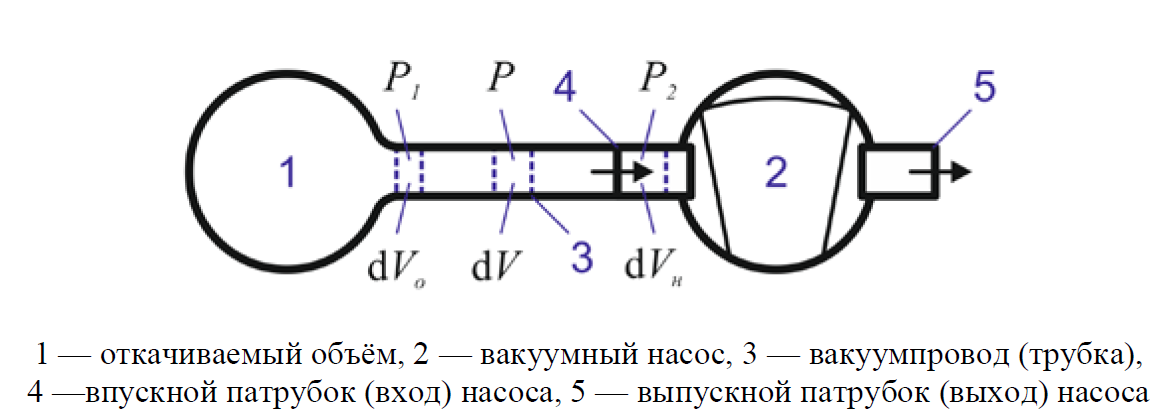
\includegraphics[width = \textwidth]{2.png}
\caption{Простейшая вакуумная система}
\label{ris2}
\end{figure}
Здесь и далее $L$ - единица измерения длины, $M$ - единица измерения массы, $T$ - единица измерения времени.
\begin{enumerate}
\item \textbf{Предельное остаточное давление} (предельный вакуум) $P_{\text{пр}} [L^{-1}MT^{-2}]$ -- наименьшее давление газа, которое формируется в процессе откачки в рассматриваемом сечении вакуумпровода (рассматриваемой точке вакуумной системы). Обычно выделяют предельное давление в камере или на входе в насос.
\item \textbf{Наибольшее выпускное давление} $[L^{-1}MT^{-2}]$ - максимально допустимое давление газа на входе насоса.
\item \textbf{Быстрота откачивающего действия} (скорость откачки) вакуумной системы $S [L^3T^{-1}]$ -- объем газа, проходящий через рассматриваемое сечение вакуумпровода в единицу времени при текущем давлении в данном сечении:
\[S = \dfrac{dV}{dT}.\]
Следовательно быстродействие насоса $S_{\text{н}}$ определяется как:
\[ S_{ \text{н} } = \dfrac{dV_{ \text{н} }}{ dt }.\]
А эффективная скорость откачки камеры $S_0$:
\[S_0 = \dfrac{ dV_0 }{ dt }.\]
\item Падение давления вдоль вакуумпровода $ \Delta P = P_1 - P_2 $ определяется его \textbf{пропускной способностью} (проводимостью) $ U [L^3 T^{-1} ] $:
\[ U = \dfrac{Q}{P_1 - P_2}, \]
где $Q [L^2 M T^{-3}]$ -- \textbf{поток газа} через вакуумпровод с соответствующими давлениями на концах.
\item Величина $Z [L^{-3}T]$, обратная проводимости, называется \textbf{импедансом} вакуумпровода:
\[Z=\dfrac{1}{U}.\]
В общем случае указанные величины $S$, $U$, $Q$, $Z$ как и сами давления $P_1$ и $P_2$ зависят от времени. Но в конце процесса откачки устанавливается квазистационарный режим, при котором поток газа становится практически постоянным и равным количеству поступающего в систему газа в единицу времени вследствие наличия течей, т.е. нарушения герметичности (в основном в местах механического соединения отдельных узлов вакуумной системы). Для стационарного режима можно записать условие непрерывности потока откачиваемого газа:
\[P_1 S_0 = PS = P_2 S_{\text{н}} = Q. \]
\item \textbf{Основное уравнение вакуумной техники}
\begin{equation}\label{main}
\dfrac{1}{S_0} = \dfrac{1}{S_{ \text{н} }} + \dfrac{1}{U}.
\end{equation}
\item Количественной характеристикой течи, является \textbf{натекание} $Q_н [L^2MT^{-3}]$, измеряемое при отключенных средствах откачки:
\[Q_н = \frac{P_к - P_н}{\Delta{t}},\]
где $V$ -- замкнутый исследуемый объём; $P_н, P_к$ -- начальное и конечное
давление в объеме; $\Delta{t}$ -- время между измерениями давления. При наличии течей, нормальной работе средств откачки и отсутствии в системе источников паров или газов, зависимость потока газа через течь от времени $Q_н(t)$ носит, как правило, линейный характер.

Для заданного давления $P_1$ в замкнутом исследуемом объёме допустимым считается натекание:
\[Q_н \ll Q = P_1S_0 = P_1\frac{S_нU}{S_н + U}.\]
\end{enumerate}

На пропускную способность вакуумпровода существенно влияет
режим течения газа, который характеризуется числом Кнудсена, равным
отношению длины свободного пробега молекул в газе к характерному
линейному размеру течения:
\[Kn = \dfrac{\lambda}{d}.\]
Данная величина характеризует степень разреженности газового
потока:
\begin{itemize}
\item В \textit{гидродинамическом} (вязкостном) режиме течения ($Kn \ll 1$)
различают ламинарные и турбулентные потоки. При ламинарном
течении молекулы газа движутся по параллельным траекториям
со скоростями, мало отличающимися друг от друга. При турбулентном течении наряду с поступательным движением всей массы газа, молекулы движутся хаотически со скоростями, подвергающимися случайным изменениям.
\item В \textit{молекулярном} (кнудсеновском) режиме ($Kn \gg 1$) течение газа
сводится к независимому движению отдельных молекул по прямым линиям в периоды между соударениями главным образом со
стенками вакуумпровода.
\item В \textit{переходном} режиме ($Kn \sim 1$) в системе могут существовать все
описанные выше виды течения.
\end{itemize}

В разных режимах течения пропускная способность вакуумпровода имеет существенно различные зависимости от размера его поперечного сечения.

\subsection{Процесс откачки}
Опишем процесс откачки математически: 
Пусть W --- объем газа, удаляемого из сосуда при данном давлении за единицу времени, $Q_i$ для различных значений i обозначим различные притоки газа в сосуд (в единицах PV), такие как течи извне $Q_\text{и}$, десорбция с поверхностей внутри сосуда $Q_\text{д}$, обратный ток через насос $Q_\text{н}$. Тогда, приравнивая убыль газа из сосуда (с точностью до $RT/\mu$) в единицу времени $-VdP$ и сумму перечисленных токов имеем:
 \begin{equation}\label{1}
 	-VdP = (PW - \sum_i Q_i)dt
 \end{equation}
 При достижении предельного вакуума устанавливается давление $P_{\text{пр}}$, и $dP = 0$. Тогда
 \begin{equation}\label{2}
 	 W = ( \sum_i Q_i )/P_{\text{пр}}
 \end{equation}
 Поскольку обычно $Q_\text{и}$ постоянно, а $Q_\text{н}$ и $Q_\text{д}$ слабо зависят от времени, также считая постоянной W, можем проинтегрировать \eqref{1} и получить:
 \begin{equation}\label{3}
 	P - P_{\text{пр}} = (P_0 - P_{\text{пр}})\exp(-\frac{W}{V}t)
 \end{equation}
Полная скорость откачки $W$, собственная скорость откачки насоса $W_{\text{н}}$ и проводимости элементов системы $C_1, C_2,...$ соотносятся согласно данной формуле, и это учтено в конструкции установки.
 \begin{equation}\label{4}
 \frac{1}{W} = \frac{1}{W} + \frac{1}{C_1} + \frac{1}{C_2} + ...
\end{equation}

\subsection{Течение газа через трубу}
Характер течения газа существенно зависит от соотношения между размерами системы и длиной свободного пробега молекул. При атмосферном и форвакуумном давлениях  длина свободного пробега меньше диаметра трубок, и течение газа определяется его вязкостью, т.е. взаимодействием молекул. При высоком вакууме течение существеннее определяется взаимодействием со стенками \\

Для количества газа, протекающего через трубу длины $l$ и радиуса $r$ в условиях высокого вакуума, справедлива формула:
\begin{equation}\label{5}
	\frac{d(PV)}{dt} = \frac{4}{3}r^3\sqrt{\frac{2\pi RT}{\mu}}\frac{P_2 - P_1}{l}
\end{equation}
Если труба соединяет насос установку, то давлением $P_1$ у насоса можно пренебречь. Давление в сосуде $P = P_2$. Тогда имеем:
\begin{equation}\label{6}
C_\text{тр} = \left(\frac{dV}{dt}\right)_\text{тр} = \frac{4r^3}{3l}\sqrt{\frac{2\pi RT}{\mu}}
\end{equation}
Для пропускной способности отверстий имеется формула
\begin{equation}\label{7}
C_\text{отв} = \left(\frac{dV}{dt}\right)_\text{отв} = S\frac{\bar{\upsilon}}{4}
\end{equation}
Для воздуха при комнатной температуре $\bar{\upsilon}/4 = 110~\text{м/с} = 11~\text{л/c}\cdot\text{см}^2$.

\section{Методика измерений}

В данной работе используются традиционные методы откачки механическим форвакуумным насосом до давления $10^{-2}$ торр и диффузионным масляным насосом до давления $10^{-4}$ торр. \\

Установка изготовлена из стекла, и состоит из форвакуумного баллона (ФБ),высоковакуумного диффузионного насоса (ВН), высоковакуумного баллона (ВБ), масляного (М) и ионизационного (И) манометров, термопарных манометров ($\text{М}_1$ и $\text{М}_2$), форвакуумного насоса (ФН) и соединительных кранов ($K_1, K_2,..., K_6$) (рис. 1). Кроме того, в состав установки входят: вариатор
 (автотрансформатор с регулируемым выходным напряжением), или
 реостат и амперметр для регулирования тока нагревателя диффузионного насоса. \\
 
  \begin{figure}[!h]
 	\centering
 	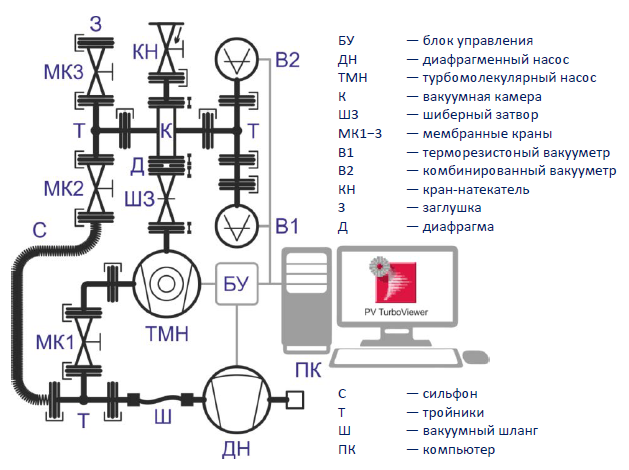
\includegraphics[width=0.5\linewidth]{3.png}
 	\caption[]{Схема установки}
 	\label{fig:Схема установки}
 \end{figure}
 
 Все краны вакуумной установки стеклянные. Стенки кранов тонкие, пробки кранов полые и составляют одно целое с рукоятками. Пробки кранов притерты к корпусам. Для герметизации используется вакуумная смазка. \\
 
 Устройство и принцип действия \textit{форвакуумного насоса} схематически, но довольно ясно изображены на рис 2. В положениях <<а>> и <<б>> пластина <<А>> засасывает разреженный воздух из откачиваемого объёма, а пластина <<Б>> вытесняет ранее захваченный воздух в атмосферу. В положениях <<в>> и <<г>> пластины поменялись ролями.
 
\begin{figure}[!h]
	\centering
	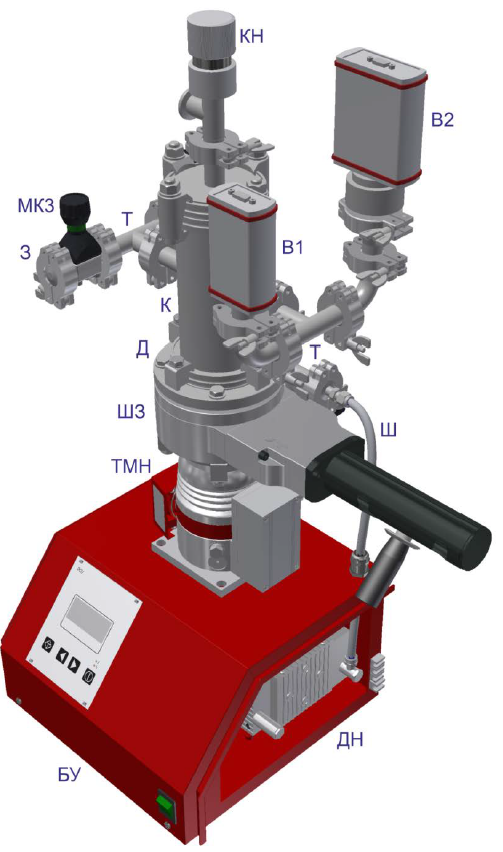
\includegraphics[width=0.9\linewidth]{4.png}
	\caption[]{Схема действия ротационного двухпластинчатого форвакуумного насоса}
	\label{fig:Схема ФВ насоса}
\end{figure}

Устройство и принцип действия \textit{диффузионного насоса} схематически изображены на рис 2. Такой насос работает в тысячи раз быстрее форвакуумного. Его действие основано на диффузии. Масло, налитое в сосуд А, подогревается электрической печкой. Пары масла поднимаются по трубке Б и вырываются из сопла В. Струя паров увлекает молекулы газа, которые поступают из откачиваемого сосуда через трубку ВВ. В трубке Г мало осаждается и стекает вниз. Оставшийся газ, выходя в трубку ФВ, откачивается форвакуумным насосом. \\

\begin{figure}[!h]
	\centering
	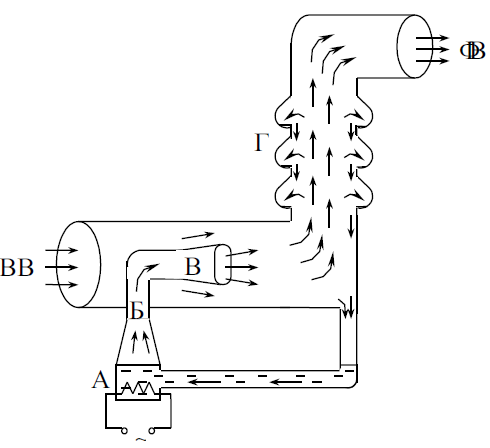
\includegraphics[width=0.4\linewidth]{5.png}
	\caption[]{Схема работы диффузионного насоса}
	\label{fig:Схема ВВ насоса}
\end{figure}

Диффузионный насос работает наиболее эффективно, когда длина свободного пробега молекул примерно равна ширине кольцевого зазора между соплом В и стенками трубки ВВ. Давление насыщенных паров масла при рабочей температуре, создаваемой обогревателем сосуда А, много больше $5\cdot 10^{-2}$ торр, поэтому пары масла создают плотную струю, увлекающую с собой молекулы газа.

\begin{wrapfigure}{r}{50mm}
 	\begin{center}
 		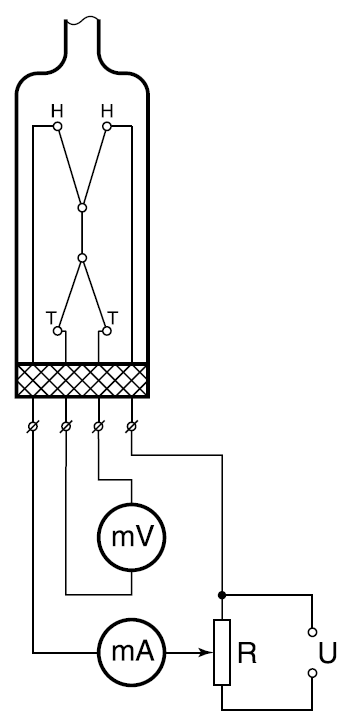
\includegraphics[width=0.8\linewidth]{6.png}
 		\caption{Схема термопарного манометра с лампой ЛТ-2}
 		\label{fig:Схема термопары}
 	\end{center}
 \end{wrapfigure}
 
Диффузионный насос, используемый в нашей установке (см. рис 1) имеет две ступени и соответственно два сопла. Одно сопло вертикальное (первая ступень), второе горизонтальное (вторая ступень). За второй ступенью имеется ещё одна печь, но пар из этой печи поступает не в сопло, а по тонкой трубке подводится ближе к печке первой ступени.
Эта печь осуществляет фракционирование масла. Легколетучие фракции масла, испаряясь, поступают в первую ступень, обогащая её. По этой причине плотность струи первой ступени выше, и эта ступень начинает откачивать при более высоком давлении в форвакуумной части. Вторая ступень обогащается малолетучими фракциями масла. Плотность струи второй ступени меньше, но меньше и давление насыщенных паров. Соответственно, в откачиваемый объем поступает меньше паров масла, и его удаётся откачать до более высокого вакуума.  \\
 
 \textit{Термопарный манометр.} Чувствительным элементом манометра является платиново-родиевая термопара, спаянная с никелевой нитью накала и заключённая в стеклянный баллон. Устройство термопары пояснено на рис. 4. По нити накала НН пропускается ток постоянной величины. Для установки тока служит потенциометр R, расположенный на передней панели вакуумметра. Термопара ТТ присоединяется к милливольтметру, показания которого определяются температурой нити накала и зависят от отдачи тепла в окружающее пространство. \\
 
 Потери тепла определяются теплопроводностью нити и термопары, теплопроводностью газа, переносом тепла конвективными потоками газа внутри лампы, и теплоизлучением нити (инфракрасное тепловое излучение). В обычном режиме лампы основную роль играет теплопроводность газа. При давлениях, не меньших 1 торр, теплопроводность газа, а вместе с ней и ЭДС термопары практически не зависят от давления газа, и прибор не работает. \\

 \begin{figure}[!h]
 	\centering
 	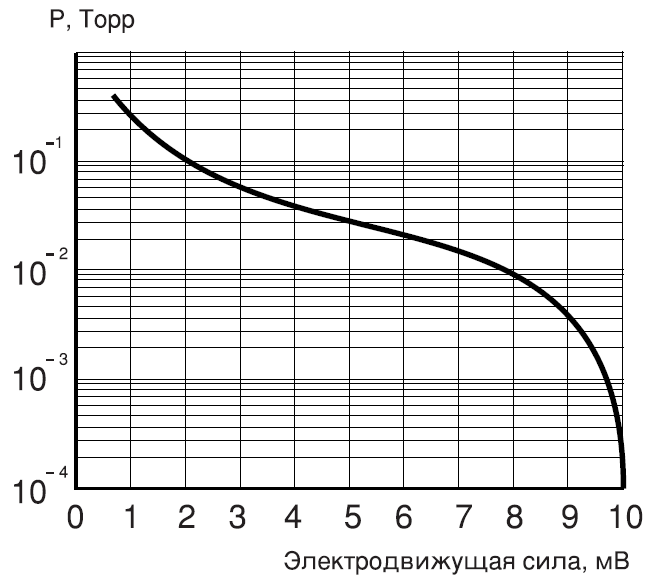
\includegraphics[width=0.5\linewidth]{7.png}
 	\caption[]{Градуировочная кривая термопары ЛТ-2}
 	\label{fig:Градуировочная кривая}
 \end{figure}

 \begin{wrapfigure}{r}{50mm} %если не лезет, но с новой стр
	\begin{center}
		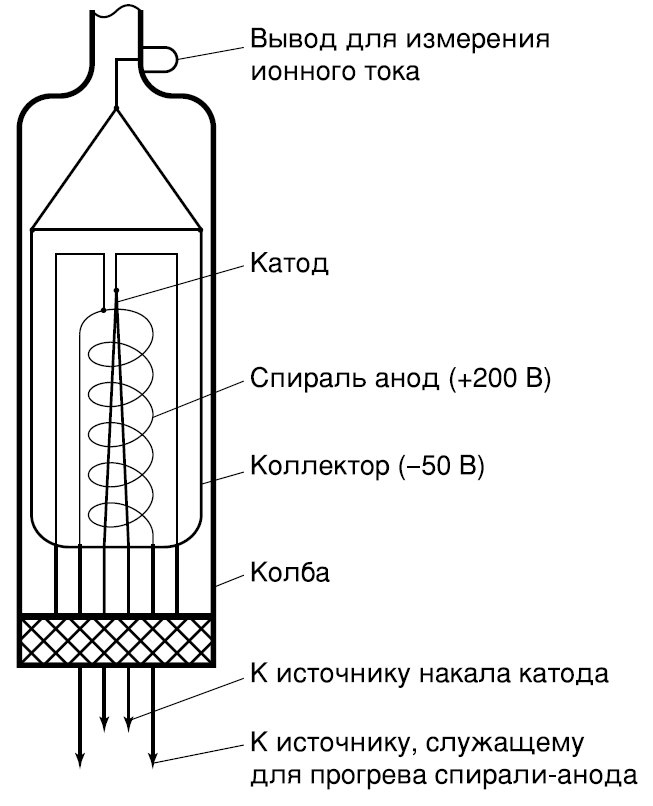
\includegraphics[width=\linewidth]{8.png}
		\caption{Схема ионизационной лампы ЛТ-2}
		\label{fig:лампа}
	\end{center}
\end{wrapfigure}

 При улучшении вакуума средний свободный пробег молекул становится сравнимым с диаметром нити, теплоотвод падает, и температура спая возрастает. При вакууме порядка $10^{-3}$ торр теплоотвод, осуществляемый газом, становится сравнимым с другими потерями тепла, и температура становится практически постоянной. Градуировочная кривая термопары приведена на рис. 5. \\

\textit{Ионизационный манометр.} Схема ионизационного манометра изображения на рисунке 6. Он представляет собой трехэлектродную лампу. Электроны испускаются раскалённым катодом и увлекаются электрическим полем к аноду, имеющему вид редкой спирали. Проскакивая за её витки, электроны замедляются полем коллектора и возвращаются к аноду. Прежде чем осесть на аноде, они успевают много раз пересечь пространство между катодом и коллектором. На своём пути электроны ионизуют молекулы газа. Ионы, образовавшиеся между анодом и коллектором, притягиваются полем коллектора и определяют его ток. \\

  Накалённый катод ионизационного манометра перегорает, если давление в системе превышает $10^{-3}$ торр, поэтому перед его включением необходимо проверить давление термопарным манометром. \\


\section{Используемое оборудование}

\begin{enumerate}
    \item Вакуумная установка с манометрами: масляными, термопарными и ионизационными, $\delta_{масл. маном.} = 0,05~см$;
\end{enumerate}

\section{Результаты измерений и обработка данных}

Начальные условия и параметры установки:

$\begin{aligned}
& P_{\text{атм}} = 101,1\pm0,05~кПа\\
& V_{K5+K6+кап} = 50~см^3 \\
& L = 10,8~см \\
& d_{кап} = 0,8~мм \\
& \rho_{масла} = 0.885~г/см^3
\end{aligned}$\\[0,5 cm]

\subsection{Определение объёма форвакуумной и высоковакуумной частей установки}

Показания масляного манометра, когда воздух <<заперт>> в форвакуумной части установки:

$\begin{aligned}
& h_1 = 34,5~см \\
& h_2 = 9~см \\
& \Delta{h_{фв}} = 25,5~см \\
\end{aligned}$\\[0,5 cm]

Тогда
\[P_{фв} = \rho g\Delta{h_{фв}} = 2211,6\pm4,3~Па.\]

По закону Бойля-Мариотта
\[P_{фв}V_{фв} = P_{атм}V_{кап} \Rightarrow V_{фв} = \frac{P_{атм}V_{кап}}{P_{фв}}.\]

Погрешность определяется по формуле
\[\delta_{V_{фв}} = \sqrt{\left(\frac{\delta_{P_{атм}}}{P_{атм}}\right)^2 + \left(\frac{\delta_{P_{фв}}}{P_{фв}}\right)^2} \cdot V_{фв}.\]

Полученное значение $V_{фв} = 2,286\pm0,005~л$.

Показания масляного манометра, когда воздух распространился по всему объёму установки:

$\begin{aligned}
& h_3 = 30,4~см \\
& h_4 = 14,1~см \\
& \Delta{h_{полн}} = 16,3~см \\
\end{aligned}$\\[0,5 cm]

Тогда
\[P_{полн} = 1413,7\pm4,3~Па.\]

Полученное значение $V_{полн} =3,576\pm0,011~л$. Следовательно, $V_{вв} = V_{полн} - V_{фв} = 1,290\pm0,012~л$.

\subsection{Получение высокого вакуума и измерение скорости откачки}

Предельное давление, достигнутое при откачке $P_{пр} = 1,6 \cdot 10^{-4}~мм.рт.ст.$ Найдём скорость откачки. Прологарифмируем формулу \eqref{3}, чтобы получить на графике прямую линию. График зависимости представлен на рис. \ref{ris3}.

\begin{figure}[h!]
\begin{flushleft}
    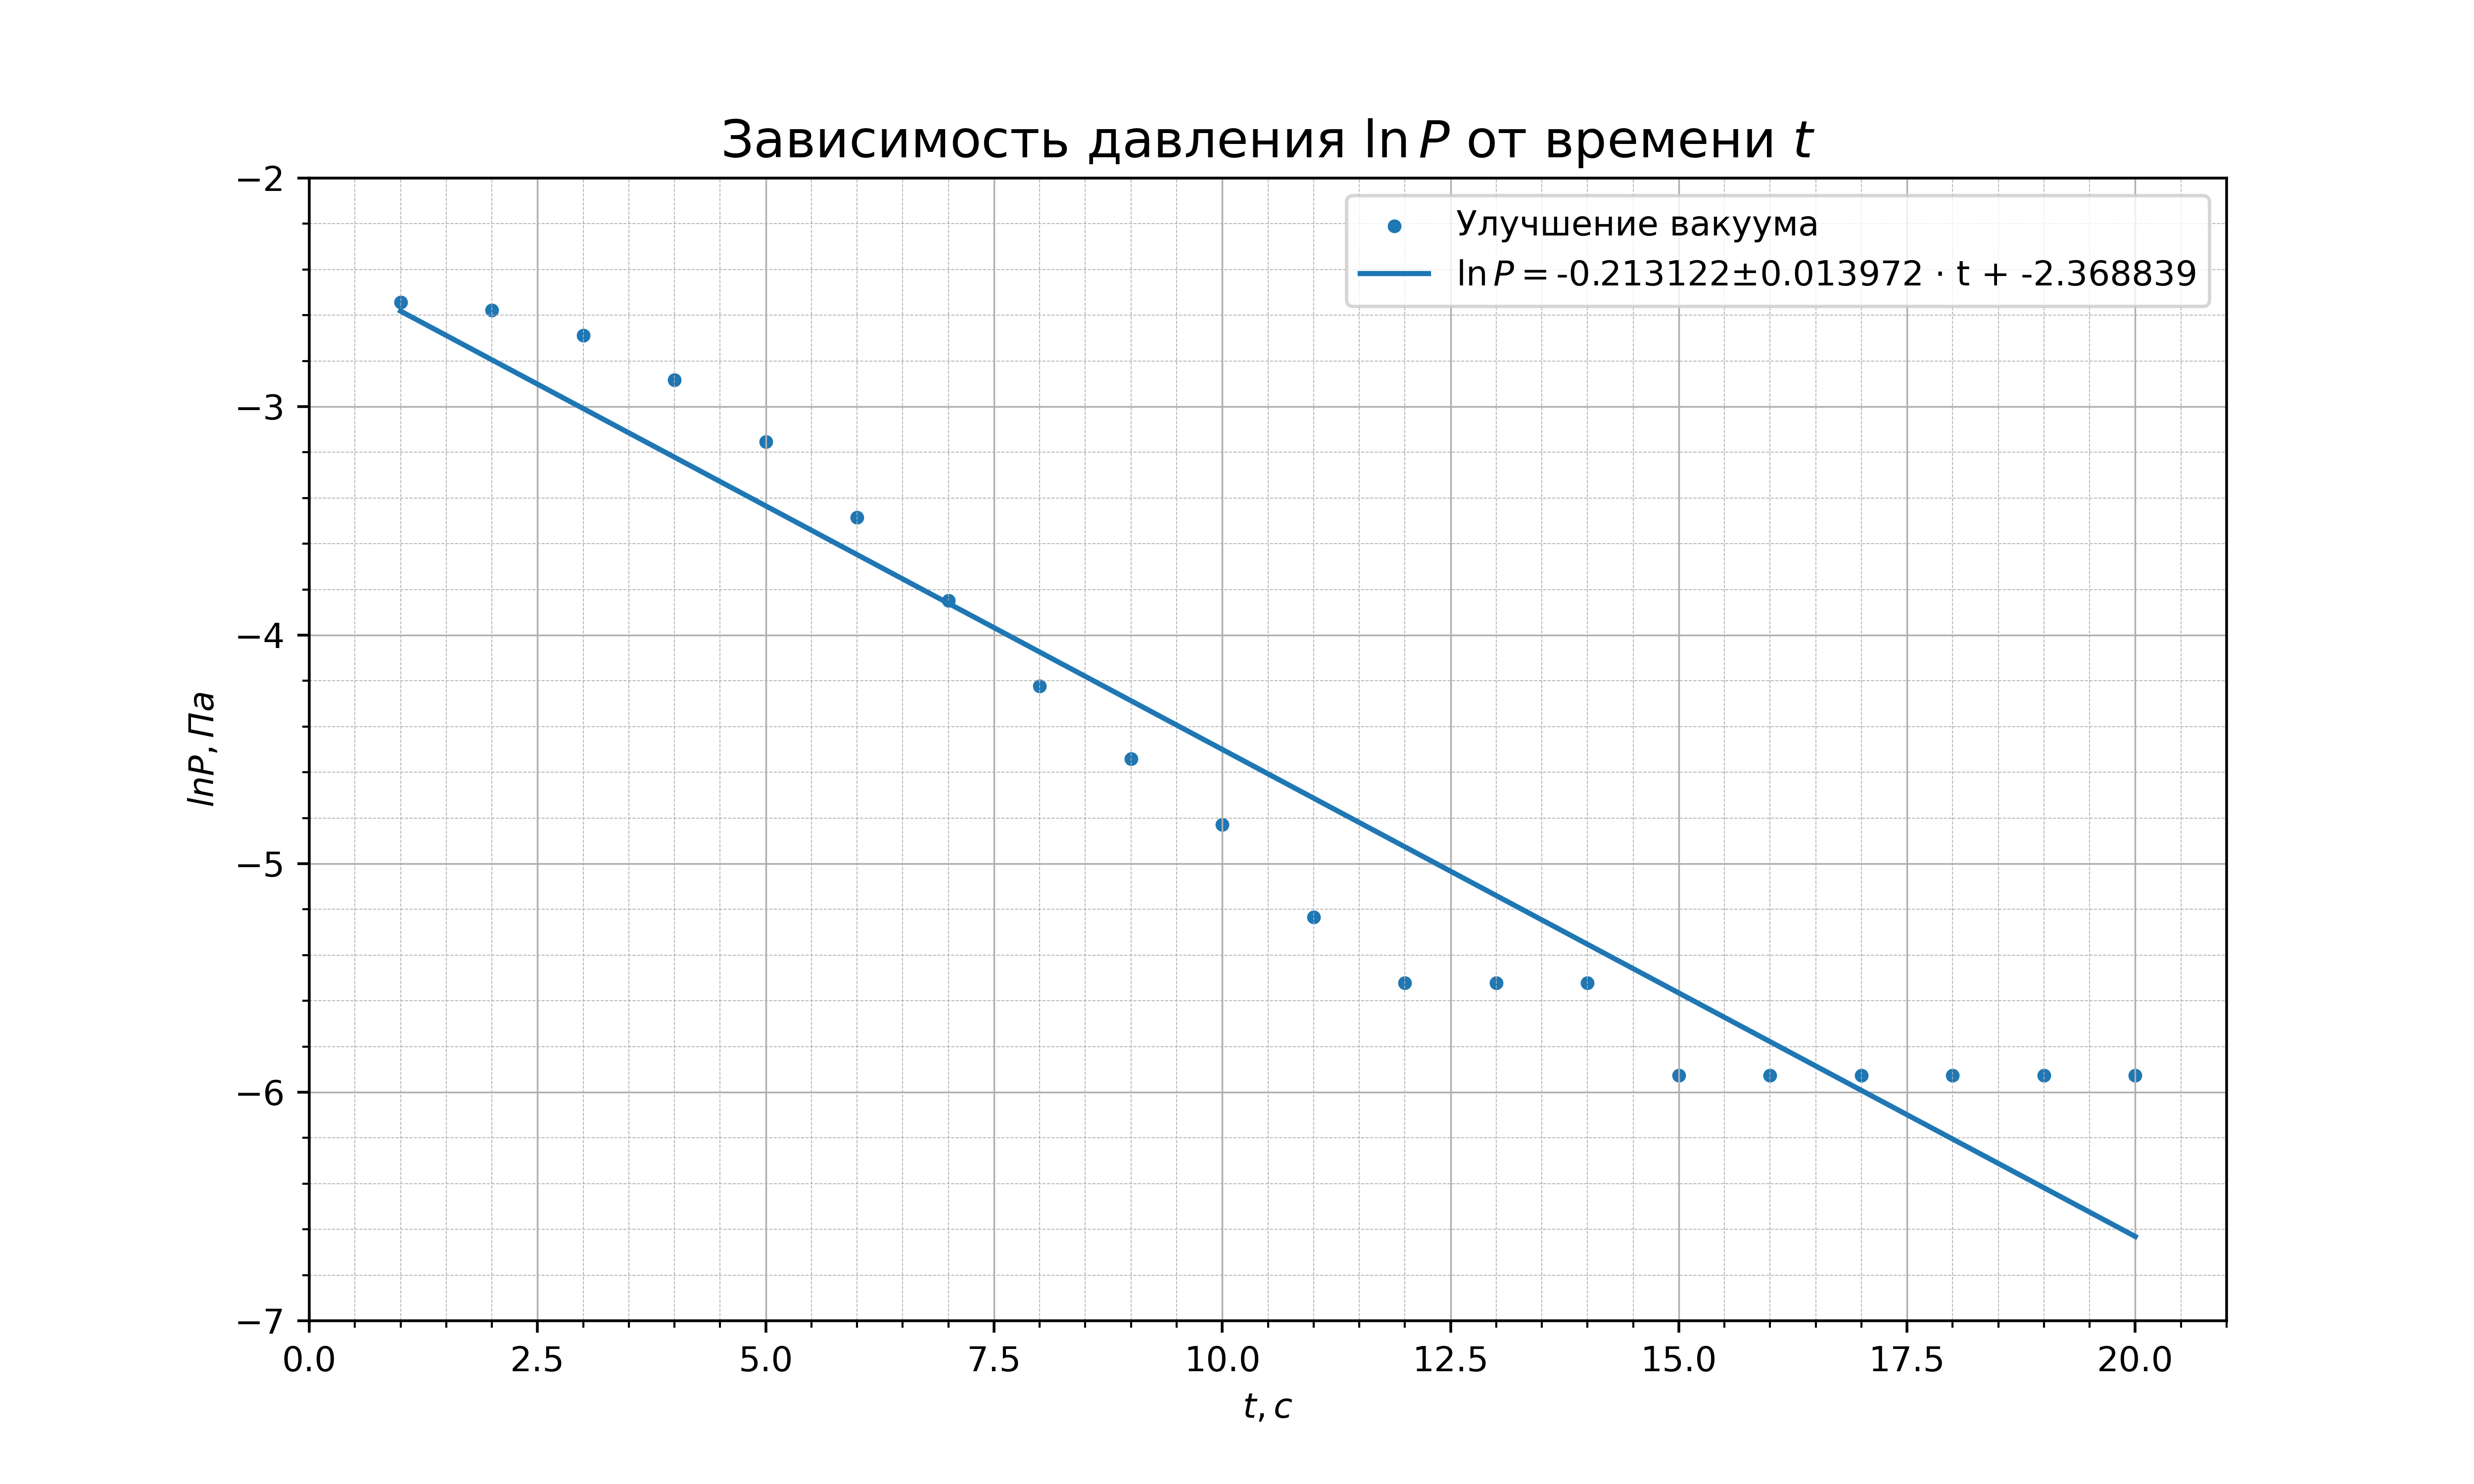
\includegraphics[scale=0.75]{2.3.1_1.png}
\end{flushleft}
\caption{}
\label{ris3}
\end{figure}

Скорость откачки определяется по формуле
\[W = -k \cdot V_{вв},\]
где $k$ --- коэффициент наклона прямой.

Погрешность определяется по формуле
\[\delta_{W} = \sqrt{\left(\frac{\delta_{k}}{k}\right)^2 + \left(\frac{\delta_{V_{вв}}}{V_{вв}}\right)^2} \cdot W.\]

Полученное значение:
\[ \boxed{W = 0,258\pm0,012~л/с}.\]

График зависимости $P$ от $t$ при ухудшении вакуума представлен на рис. \ref{ris4}.

\begin{figure}[h!]
\begin{flushleft}
    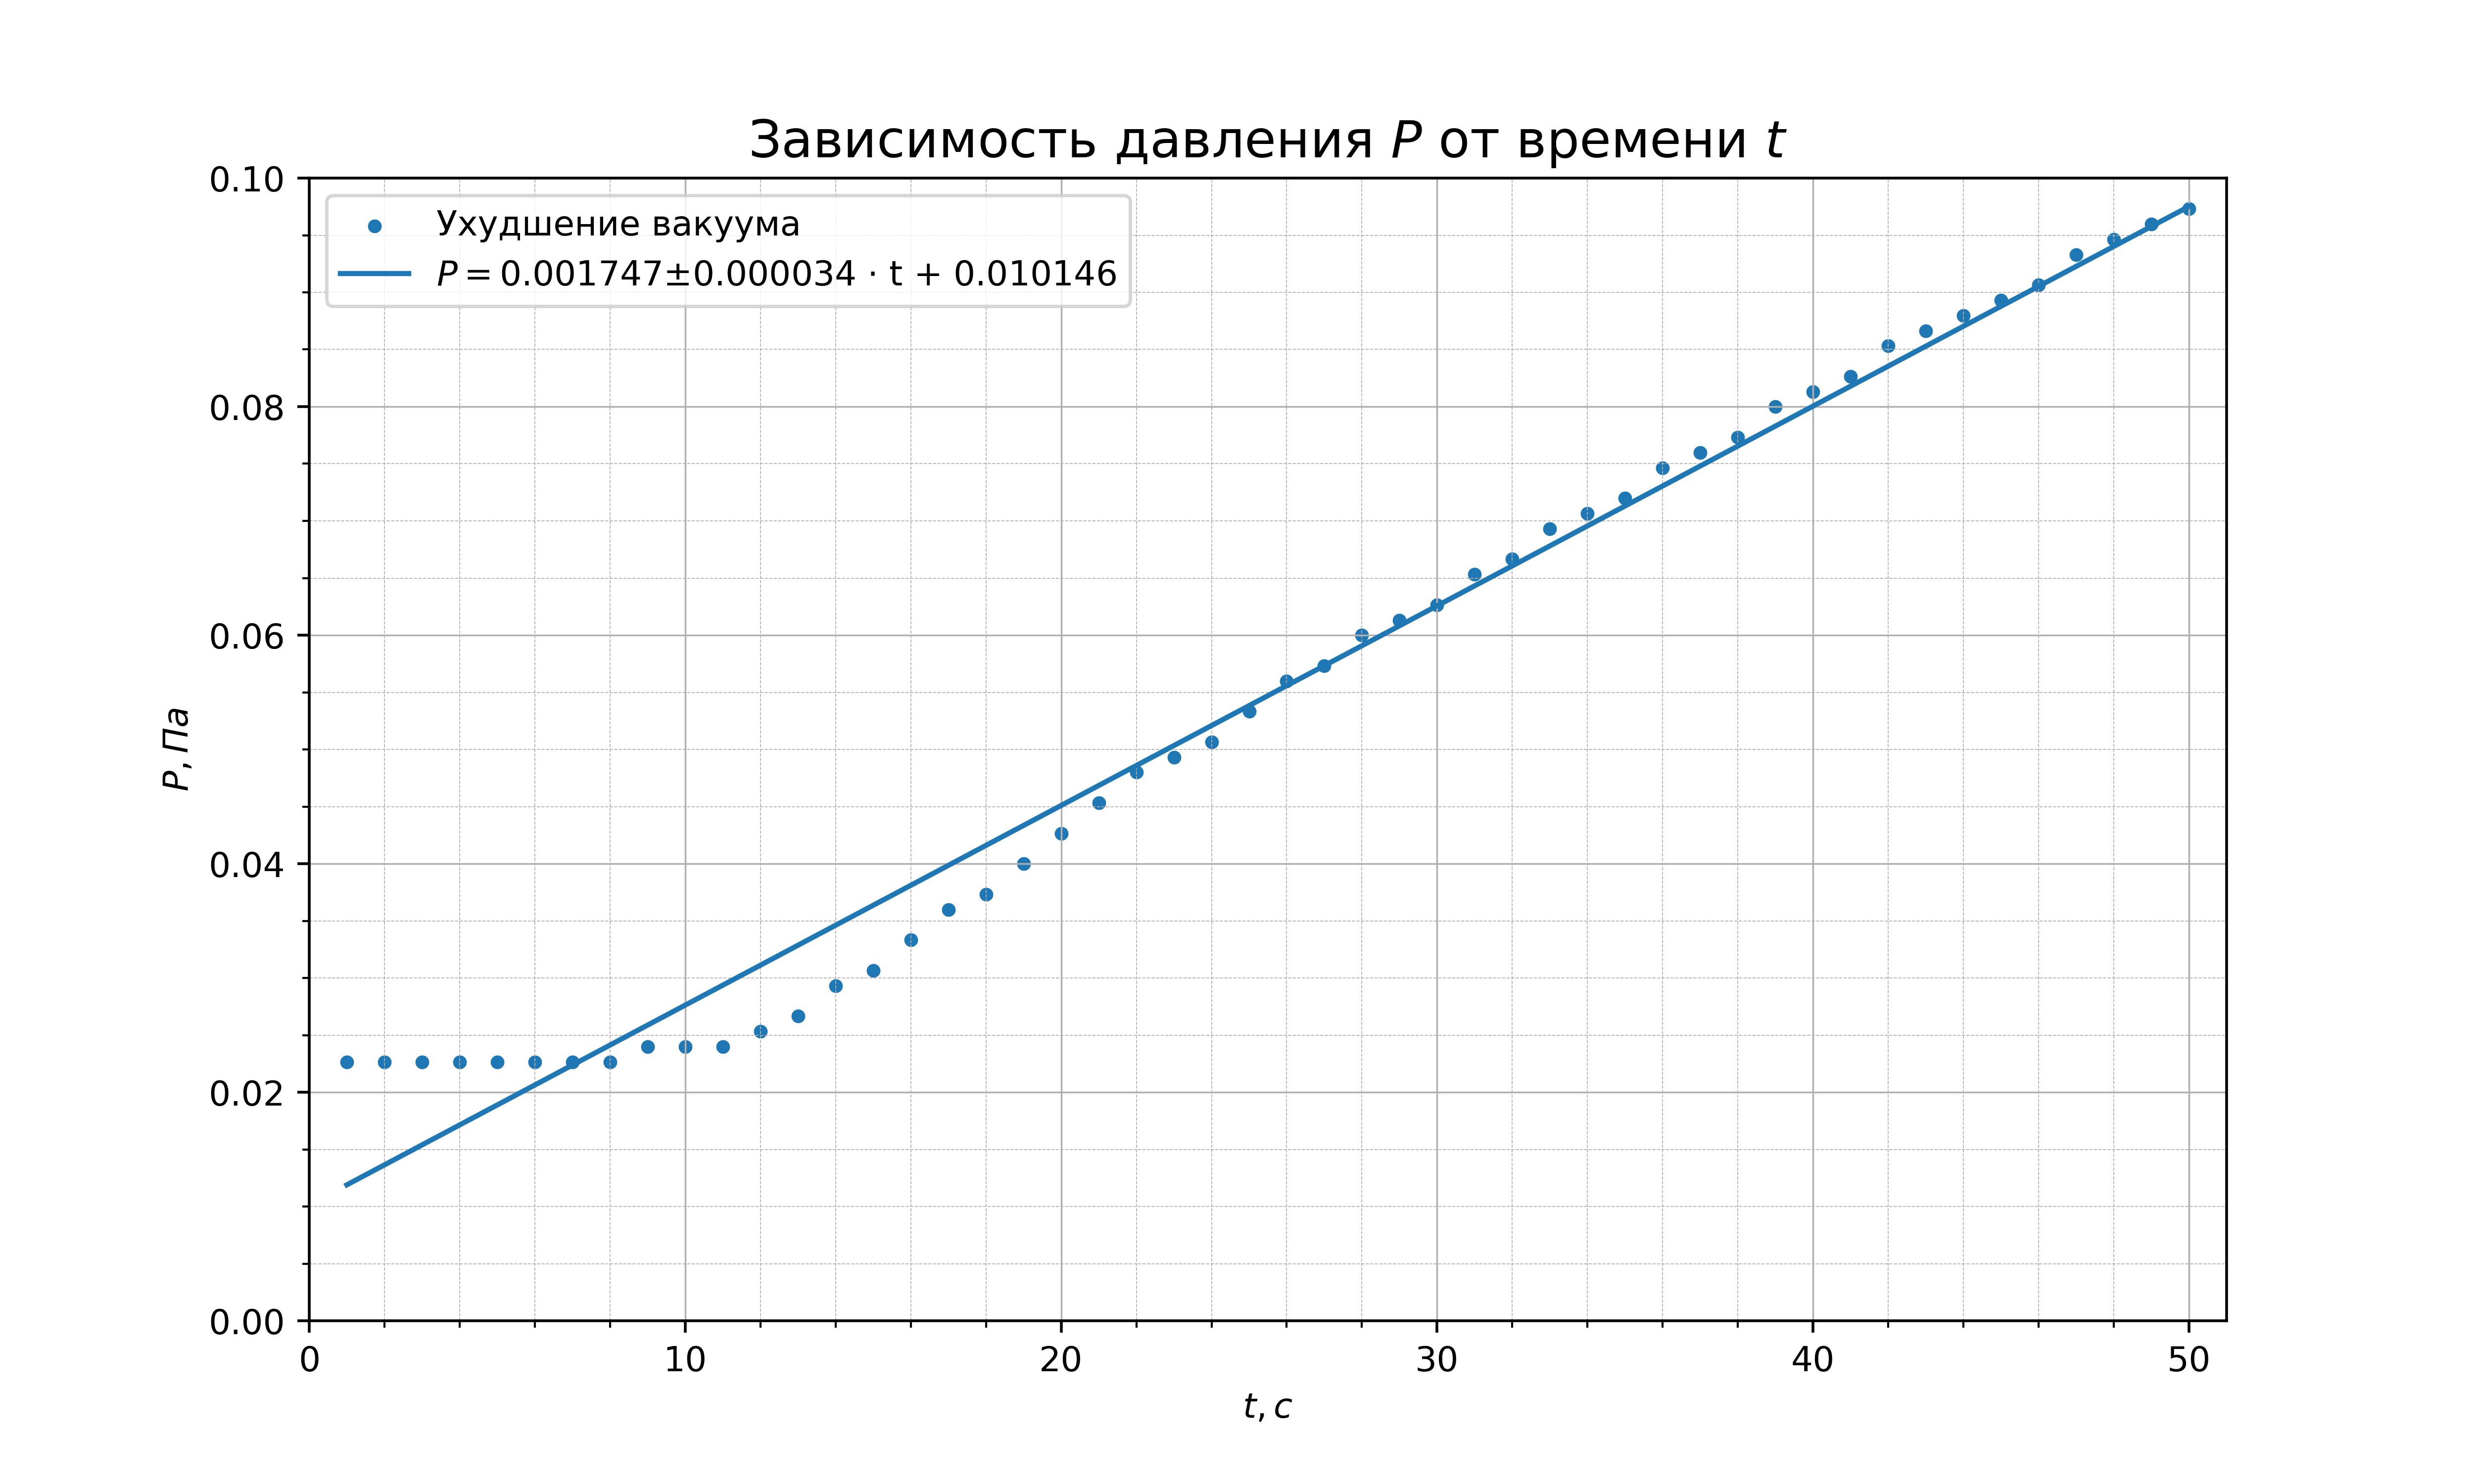
\includegraphics[scale=0.75]{2.3.1_2.png}
\end{flushleft}
\caption{}
\label{ris4}
\end{figure}

Используя соотношение \eqref{1}, которое примет вид $$V_{вв}dP = (Q_{д} + Q_{н})dt,$$ оценим $Q_{н}$. Считаем
\[\frac{dP}{dt} = k,\]
где $k$ --- коэффициент наклона прямой при ухудшении вакуума. Погрешность определяется по формуле
\[\delta_{(Q_{д} + Q_{н})} = \sqrt{\left(\frac{\delta_{k}}{k}\right)^2 + \left(\frac{\delta_{V_{вв}}}{V_{вв}}\right)^2} \cdot V_{вв}k.\]
Получаем:
\[Q_{н} + Q_{д} \approx 23,2\pm0,5 \cdot 10^{-4}~Па \cdot л/с.\]

Так как $Q_{д} \ll Q_{н}$, можно считать $Q_{д} + Q_{н} \approx Q_{н}$. Таким образом,
\[\boxed{Q_{н} \approx 23,2\pm0,5 \cdot 10^{-4}~Па \cdot л/с}.\]

Оценим пропускную способность трубы от вакуумного баллона, имея в виду порядки её диаметра и длины и размерного множителя $$d \sim 10^{-2}~м,\quad L \sim 1 ~м,\quad \sqrt{\frac{RT}{\mu}} \sim 500 ~м/с,$$ используя формулу \eqref{6} имеем:
$$C_\text{тр} \sim 1 ~л/с,$$
что отлично согласуется с полученным ранее значением $W$.

Расчитаем производительность насоса по различию $P_{уст}$ и $P_{пр}$. $$P_{уст} = 2,2 \cdot 10^{-4}~мм. рт. ст., \quad P_{фв} = 1,1 \cdot 10^{-3}~мм. рт. ст.$$

Запишем \eqref{2} для данного случая:
$$P_\text{пр}W = Q_1, \quad P_\text{уст}W = Q_1 + \frac{(PV)_{кап}}{dt}.$$

С учётом \eqref{6} получаем
$$(P_\text{уст} - P_\text{пр})W = \frac{4}{3}(d/2)^3\sqrt{\frac{2\pi RT}{\mu}}\frac{P_\text{фв}}{L},$$
где $d$ и $L$ --- диаметр и длина капилляра.
Получаем:
\[\boxed{W = 0,141\pm0,018~л/с}.\]

Результат отличается почти ровно в два раза от полученного ранее. Вероятно, потому что теперь течение газа определяется пропускной способностью двух труб, соединённых последовательно \eqref{5}. Судя по всему, проводимости трубки от ВВ баллона и капилляра сравнимы.

\section{Обсуждение результатов и выводы}

В данной работе исследовалась зависимость давления в установке от времени. По результатам измерения давления различными способами определялась производительность вакуумного насоса. Полученное значение для скорости откачки:
\[\boxed{W = 0,258\pm0,012~л/с}.\]
Использованный в работе метод измерений позволяет достичь относительной точности результатов в 5\%. Метод расчёта скорости откачки по зависимости давления от времени при улучшении вакуума оказался точнее в сравнении с методом расчёта по различию $P_{уст}$ и $P_{пр}$. Основной вклад в погрешность вносит погрешность определения коэффициентов линейной аппроксимации.
Также в данной работе были проверены теоретические зависимости, связанные с течением газа (рис. \ref{ris3} и \ref{ris4}).

\end{document}